\documentclass[tikz,border=10pt]{standalone}
\usepackage{tikz}
\usepackage{amssymb}
\usetikzlibrary{shapes.geometric, arrows.meta, positioning, calc, backgrounds, fit}

\definecolor{pbblue}{HTML}{EBF5FB}
\definecolor{pbdarkblue}{HTML}{1B4F72}
\definecolor{pbmint}{HTML}{E8F8F5}
\definecolor{pbdarkgreen}{HTML}{0E6251}
\definecolor{pblavender}{HTML}{F4ECF7}
\definecolor{pbdarkpurple}{HTML}{512E5F}
\definecolor{pbyellow}{HTML}{FEF9E7}
\definecolor{pbdarkyellow}{HTML}{7D6608}
\definecolor{pbcoral}{HTML}{FDEDEC}
\definecolor{pbdarkred}{HTML}{78281F}
\definecolor{pbgray}{HTML}{F8F9F9}

\begin{document}
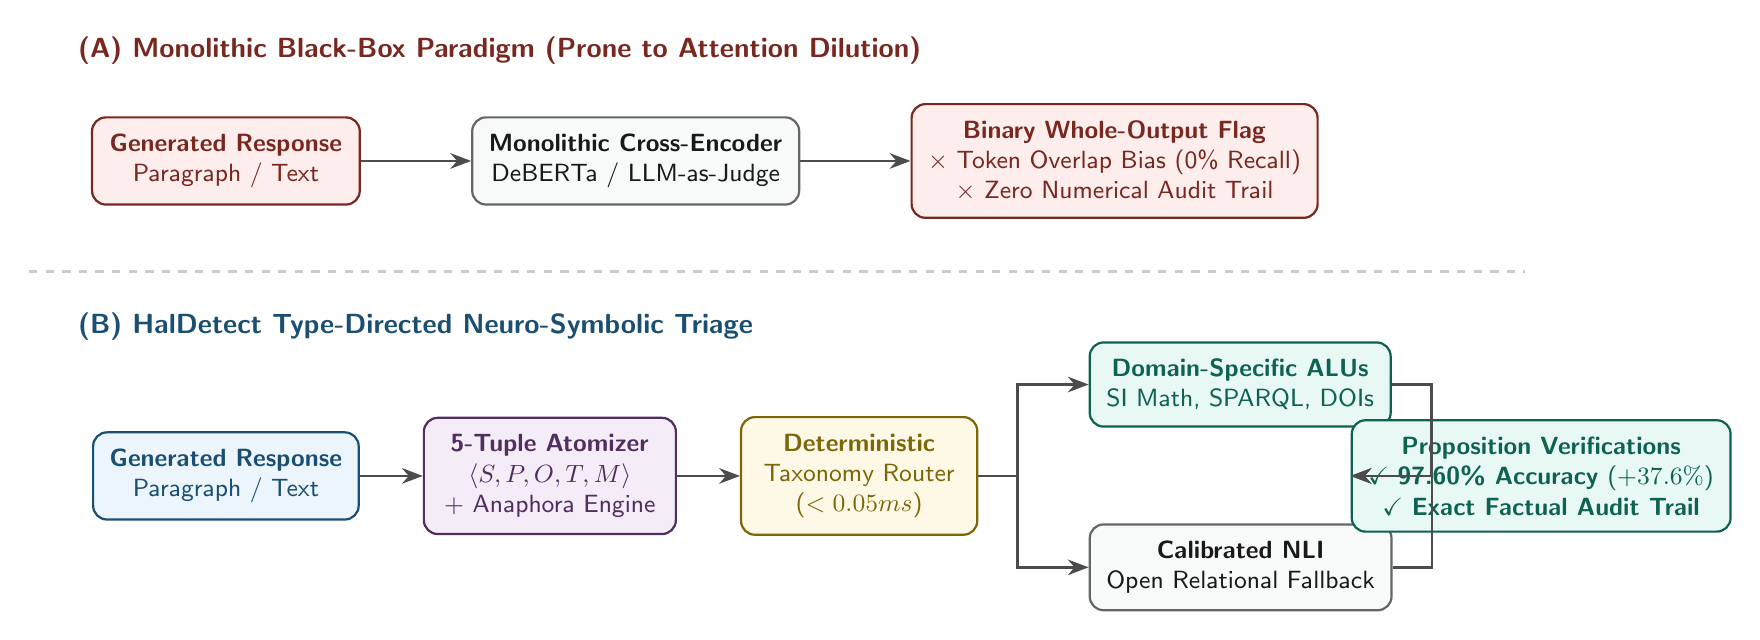
\begin{tikzpicture}[
    font=\sffamily\small,
    box/.style={draw=black!70, rounded corners=5pt, line width=0.8pt, align=center, inner sep=6pt},
    arrow/.style={-{Stealth[scale=1.0]}, line width=1.0pt, draw=black!70}
]

% ------------------- Paradigm A: Monolithic Black-Box -------------------
\node[anchor=west, font=\bfseries\sffamily\normalsize, text=pbdarkred] at (0, 4.2) {(A) Monolithic Black-Box Paradigm (Prone to Attention Dilution)};

\node[box, fill=pbcoral, draw=pbdarkred, text=pbdarkred, minimum width=3.4cm] (a_input) at (2.0, 2.8) {\textbf{Generated Response}\\Paragraph / Text};
\node[box, fill=pbgray, draw=black!60, text=black!90, right=1.4cm of a_input, minimum width=3.8cm] (a_judge) {\textbf{Monolithic Cross-Encoder}\\DeBERTa / LLM-as-Judge};
\node[box, fill=pbcoral, draw=pbdarkred, text=pbdarkred, right=1.4cm of a_judge, minimum width=4.2cm] (a_output) {\textbf{Binary Whole-Output Flag}\\$\times$ Token Overlap Bias (0\% Recall)\\$\times$ Zero Numerical Audit Trail};

\draw[arrow] (a_input) -- (a_judge);
\draw[arrow] (a_judge) -- (a_output);

\draw[dashed, gray!40, line width=1.0pt] (-0.5, 1.4) -- (18.5, 1.4);

% ------------------- Paradigm B: HalDetect Neuro-Symbolic -------------------
\node[anchor=west, font=\bfseries\sffamily\normalsize, text=pbdarkblue] at (0, 0.7) {(B) HalDetect Type-Directed Neuro-Symbolic Triage};

\node[box, fill=pbblue, draw=pbdarkblue, text=pbdarkblue, minimum width=3.2cm] (b_input) at (2.0, -1.2) {\textbf{Generated Response}\\Paragraph / Text};
\node[box, fill=pblavender, draw=pbdarkpurple, text=pbdarkpurple, right=0.8cm of b_input, minimum width=3.2cm] (b_atom) {\textbf{5-Tuple Atomizer}\\$\langle S, P, O, T, M \rangle$\\+ Anaphora Engine};
\node[box, fill=pbyellow, draw=pbdarkyellow, text=pbdarkyellow, right=0.8cm of b_atom, minimum width=3.0cm] (b_router) {\textbf{Deterministic}\\Taxonomy Router\\($< 0.05\text{ms}$)};

\node[box, fill=pbmint, draw=pbdarkgreen, text=pbdarkgreen, right=1.4cm of b_router.north east, anchor=west, yshift=0.4cm, minimum width=3.6cm] (b_alu) {\textbf{Domain-Specific ALUs}\\SI Math, SPARQL, DOIs};
\node[box, fill=pbgray, draw=black!60, text=black!90, right=1.4cm of b_router.south east, anchor=west, yshift=-0.4cm, minimum width=3.6cm] (b_nli) {\textbf{Calibrated NLI}\\Open Relational Fallback};

\node[box, fill=pbmint, draw=pbdarkgreen, text=pbdarkgreen, right=1.4cm of $(b_alu)!0.5!(b_nli)$, minimum width=3.8cm] (b_final) {\textbf{Proposition Verifications}\\$\checkmark$ \textbf{97.60\% Accuracy} ($+37.6\%$)\\$\checkmark$ \textbf{Exact Factual Audit Trail}};

\draw[arrow] (b_input) -- (b_atom);
\draw[arrow] (b_atom) -- (b_router);
\draw[arrow] (b_router.east) -- ++(0.5,0) |- (b_alu.west);
\draw[arrow] (b_router.east) -- ++(0.5,0) |- (b_nli.west);
\draw[arrow] (b_alu.east) -| ++(0.5,-0.4) |- (b_final.west);
\draw[arrow] (b_nli.east) -| ++(0.5,0.4) |- (b_final.west);

\end{tikzpicture}
\end{document}